
%\begin{abstract}
% This user guide aims to help authors and editors of Language Science Press to use the book publication tool Open Monograph Press. The first chapter gives a general introduction to the press and the tool. The remaining part of the user guide is devided in a guide for the author and one for the editor.  
%\end{abstract}


%\todo[inline]{Begriffsverwirrung auflösen (editorial, copyediting, typesetting, proofreading, production)}
%\todo[inline]{Formulierungen überprüfen (Brüche zwischen meinen Formulierungen und denen von PKP?)}
%\todo[inline]{unlogische Sachen finden (Bild an falscher Stelle, Anweisung unklar, etc.)}

%\newpage

% *** Intro ********************************
 
\chapter{Background} \label{sec:intro}

Language Science Press\footnote{More Information about the Press and the underlying project: \url{http://langsci-press.org/Meta/}} "publishes high quality, peer-reviewed open-access books in the field of linguistics". To simplify and distribute the production process among different editors the press uses Open Monograph Press\footnote{Webpage of the project: \url{https://pkp.sfu.ca/omp/}, last access: 17.10.2014.} (OMP).

\begin{quote}
OMP is an open source tool for managing and publishing monographs, edited volumes, and scholarly editions over the Web. It is a highly flexible editor-operated book management and publishing system. It has been designed to reduce the time and energy devoted to the clerical and managerial tasks associated with publishing books, while improving the record-keeping and efficiency of editorial processes. It seeks to improve the scholarly and public quality of publishing through a number of innovations, and includes clear and intuitive workflows for every aspect of the manuscript submission, review, editing and production processes.\footnote{OMP Userguide: \url{http://pkp.sfu.ca/wiki/index.php/OMP_Userguide}, last access: 09.10.2014.}
\end{quote}

\begin{figure}[h] \centering

\includegraphics[width=\textwidth]{./img/workflow.jpg}
\caption{Workflow of Language Science Press}
\label{fig:workflow}
\end{figure}

Language Science Press uses OMP to support the workflow in \figref{fig:workflow}.
The process starts with the submission of a manuscript by an author. The manuscript is accepted by the editor and distributed to reviewers. After the content based review process, the form based editorial process takes place with proofreading and typesetting. The last step is the publication of the book.  

The following two chapters aim to help authors (Chapter \ref{sec:author}) and editors (Chapter \ref{sec:editor}) to use the online tool OMP with Language Science Press. This user guide is based on the OMP userguide by PKP\footnote{OMP Userguide: \url{http://pkp.sfu.ca/wiki/index.php/OMP_Userguide}, last access: 09.10.2014.}. It has been condensed, adapted to the Language Science Press workflow and screenshots from the OMP installation for Language Science Press have been added.


% *** Create an account ********************************

%\section{Create an account}

%\todo[inline]{describe register and enrollment}


\newpage

% *** Author ***********************************************************************

\chapter{Author} \label{sec:author}
As an author you can hand in a submission, follow the document throught the process and upload revisions. 

% \todo[inline, color=green!40]{Unterschied Author/Volume Editor. Autoren sind normalerweise intern konsisten ;) bei Sammelbänden ist das nicht so. Vor der Einreichung sollte der Hrsg das Manuskript glattstreichen. Ausserdem ist die Abfrage des rechtlichen Status etwas anders, also der Vertrag mit uns. Der Workflow ist dann aber in OMP gleich, nur dass der Hrsg halt diverse Sachen an die Autoren weiterleiten muss}

\section{Starting a submission} \label{sec:submission}
\begin{figure}[h] \centering
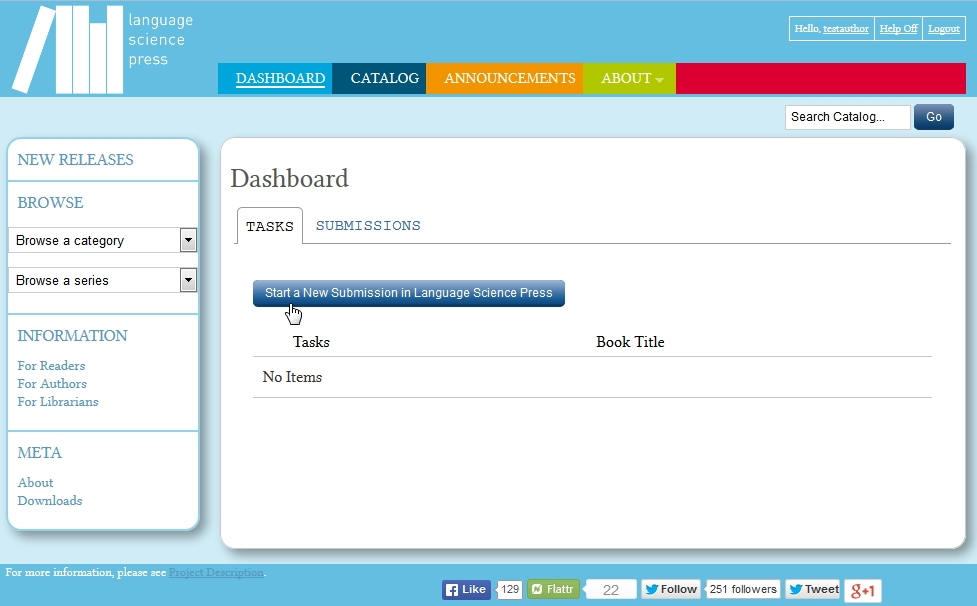
\includegraphics[width=1\textwidth]{./img/startSubmission.jpg}
\caption{Start a new submission}
\label{fig:submission}
\end{figure}
To begin the manuscript submission process, login, go to your dashboard and click the \textit{start a new submission in Language Science Press} link (\figref{fig:submission}). The submission process consists of four steps (see also  \figref{fig:submission1}): 
\begin{enumerate}[noitemsep]
\item Preparing the submission
\item Uploading the submission files
\item Providing catalog information  
\item Next Steps
\end{enumerate}

\subsection*{Step 1: Prepare}

To prepare the submission you have to agree to a number of submission checklist items (see \figref{fig:submission1}) and give general information about your submission: the type (monograph or edited Volume) and the language  of your book (see  \figref{fig:submission2}).

\begin{figure}[h]
\centering
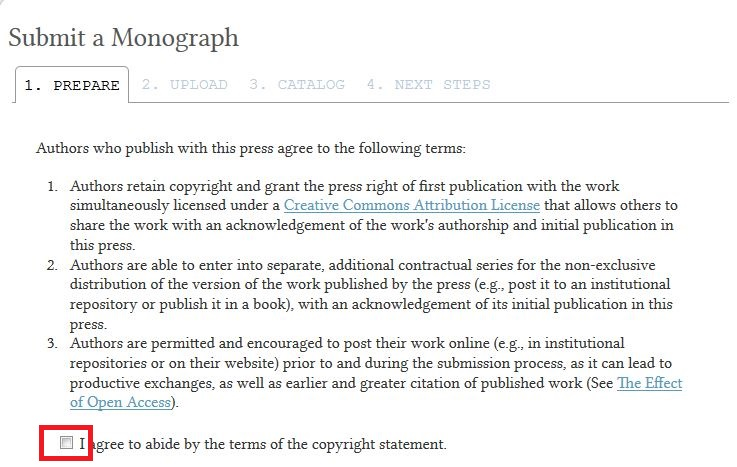
\includegraphics[width=1\textwidth]{./img/submission-1.jpg}
\caption{Prepare the Submission}
\label{fig:submission1}
\end{figure}

\begin{figure}[h]
\centering
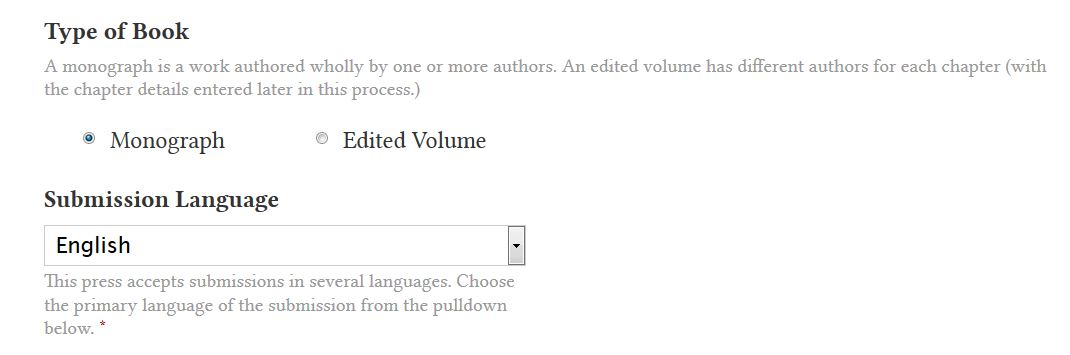
\includegraphics[width=1\textwidth]{./img/submission-2.jpg}
\caption{Set Type and Language of Book}
\label{fig:submission2}
\end{figure}

You must first choose how you will be submitting your manuscript -- for example, as an individual author, as a volume editor, as a translator, etc. -- and whether the submission is an individually-authored work, or an edited volume with multiple chapter authors. If you are submitting an edited volume, you will be able to list chapters and assign contributors to those chapters at a later stage. Authored works can also have other contributors (additional authors, translators, etc.) who are assigned to the work as a whole rather than individual chapters.


You will then be able to choose the series within which your manuscript falls (\figref{fig:submission3}). Choosing a series classifies the work into a set of related publications. Several series\footnote{More information about the projects: http://userblogs.fu-berlin.de/langsci-press/series/, last access: 09.10.2014.} are available. Confirm the checklist (see fig. \ref{fig:checklist}).

Finally, you can optionally add a cover note to the editor (\figref{fig:submission3}). Once this initial step has been accomplished, press \textit{save and continue}. Your submission is stored at your dashboard and can be completed later.

\begin{figure}[h] \centering 
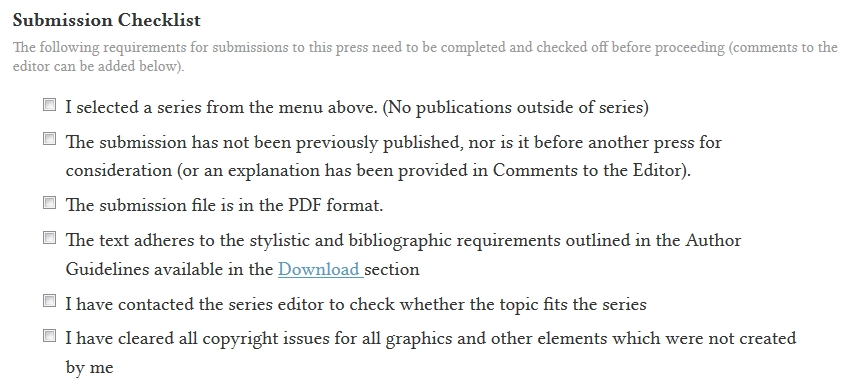
\includegraphics[width=1\textwidth]{./img/checklist.jpg} 
\caption{Checklist}
\label{fig:checklist}
\end{figure}

\begin{figure}[h]
\centering
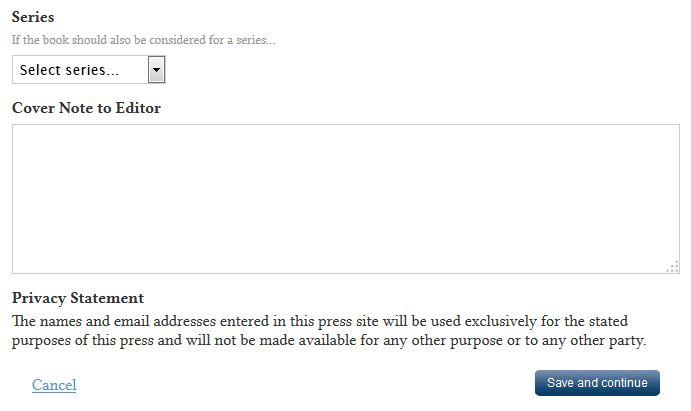
\includegraphics[width=1\textwidth]{./img/submission-3.jpg}
\caption{Choice of series and note to the editor}
\label{fig:submission3}
\end{figure}

\newpage

\subsection*{Step 2: Upload}
Upload your manuscript as a single submission file. To do so select first the content type (e.g. bibliography or book manuscript). Then you will be able to upload your file. Click \textit{continue} to add the name of the file, for example the title of your work.

% we do not need instructions for adding multiple files
%\begin{figure}[h] \centering 
%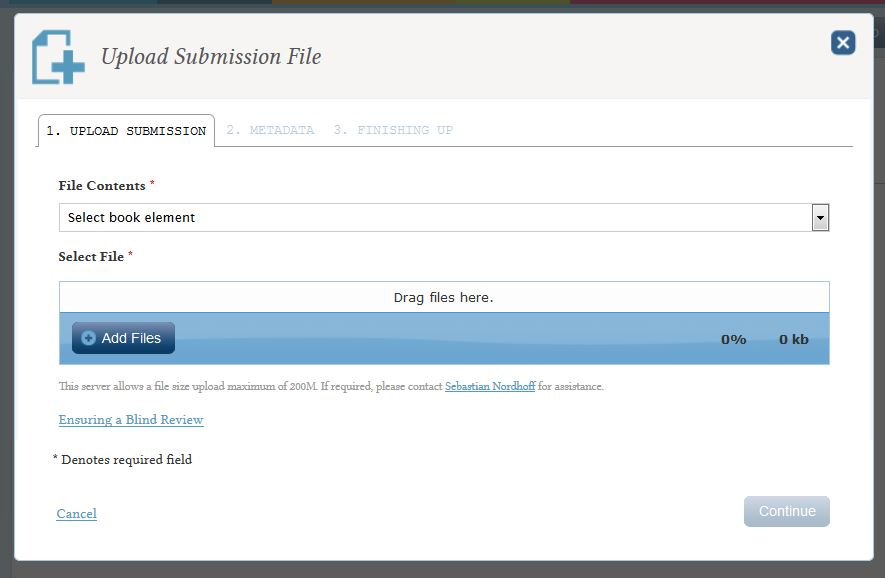
\includegraphics[width=1\textwidth]{./img/submission-4.jpg} 
%\label{fig:submission4}
%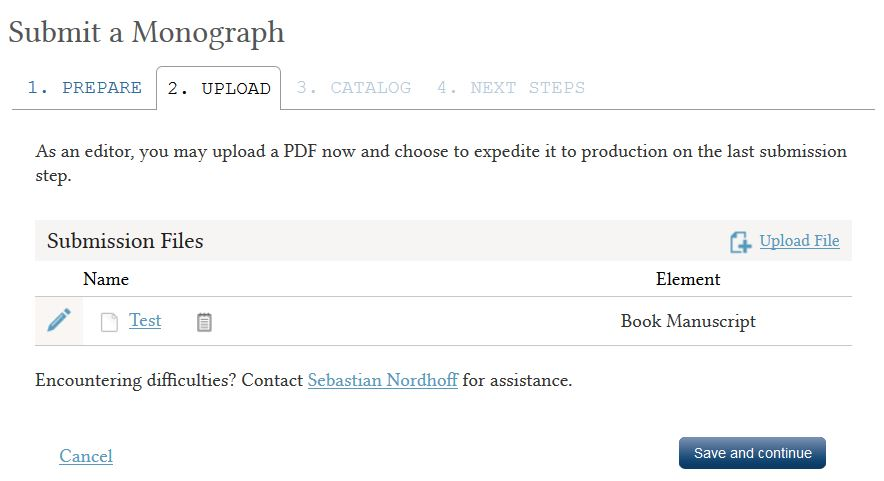
\includegraphics[width=1\textwidth]{./img/submission-5.jpg} 
%\caption{Upload submission file}
%\label{fig:submission5}
%\end{figure}

%To upload more files select \textit{submit a new file} at the end of the dialog or \textit{upload file} at the submissions overview (see fig. \ref{fig:submission5}). Once you have uploaded all relevant submission files, click \textit{save and continue}.
%

\subsection*{Step 3: Catalog}

Add information about your book at step 3: it will be included in the press catalog once the book is published. The information can be reviewed at later stages of the publication process. You must provide a submission title and an abstract, and may provide other information including a prefix, subtitle, and submission summary (\figref{fig:submission6}).

\begin{figure}[h] \centering 
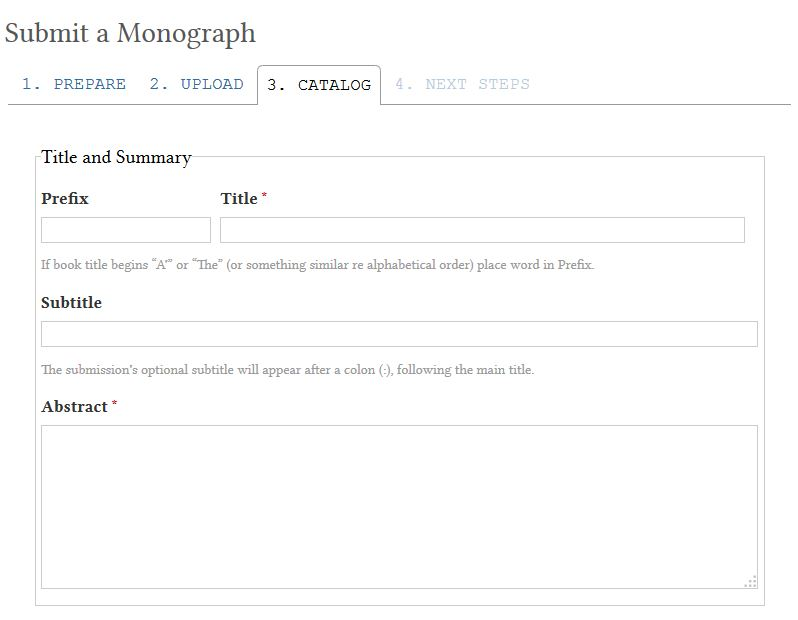
\includegraphics[width=1\textwidth]{./img/submission-6.jpg} \caption{Add Metadata}
\label{fig:submission6}

\end{figure}

Further information can be added to the submission: coverage information, submission keywords, source and rights information, and more. You can add categories from a list of given ones (\figref{fig:submission7}). You can also provide a list of contributors. The list of contributors associated with this submission may include other authors, individual chapter authors of an edited volume, volume editors, and/or translators. One contributor from the list may be assigned as the primary contact for editorial correspondence; this does not necessarily have to be the submitting author. Once you have completed this step, click \textit{finish submission}.

\begin{figure}[h] \centering 
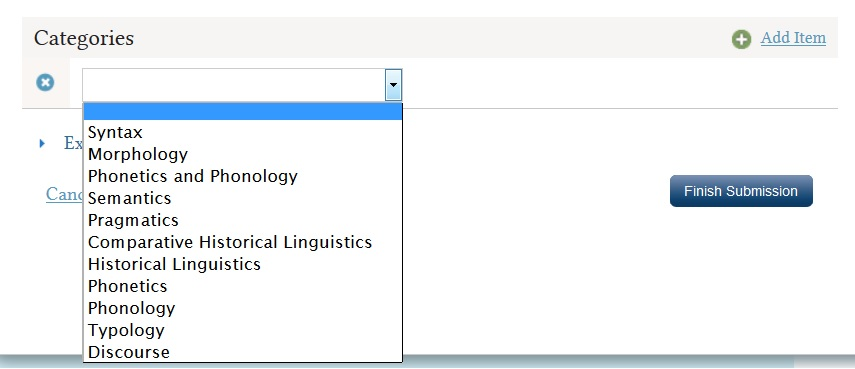
\includegraphics[width=1\textwidth]{./img/submission-7.jpg} 
\caption{Select categories}
\label{fig:submission7}
\end{figure}

\subsection*{Step 4: Next Steps}

The final step confirms that your submission has been received, and provides you with links to review your submission, create a new submission, or visit your dashboard. 

% \todo[inline]{add information about the review process from author view}

%\begin{figure}[here] \centering
%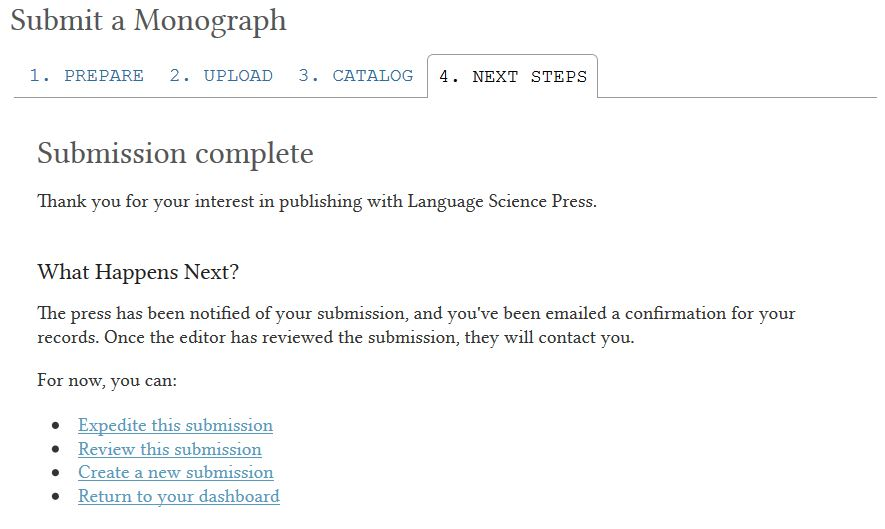
\includegraphics[width=1\textwidth]{./img/submission-8.jpg} \caption{Confirmation and Next Steps}
%\label{fig:submission8}
%\end{figure}


% *** Editor ***********************************************************************

\chapter{Editor} \label{sec:editor}

As an editor you can receive submissions, manage the review, the editorial and the production of the document (see also workflow at Chapter \ref{sec:intro}). In OMP the workflow is represented in the following steps (\figref{fig:workflowOmp}).

\begin{figure}[h] \centering
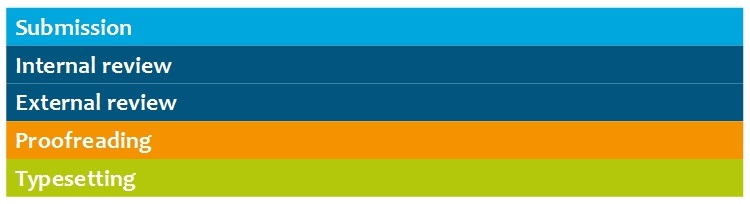
\includegraphics[width=1\textwidth]{./img/workflow_omp.jpg} \caption{Workflow in OMP}
\label{fig:workflowOmp}
\end{figure}

As an editor you manage the steps, assign reviewers and other roles. The following chapters describe each single step in detail. An overview:

\begin{itemize}
\item Submission \\receive the submission by the author and assign an editor
\item Internal review \\assign internal reviewers and external to the documtent to check the content 
\item External review \\assign external reviewers to the documtent to check the content
\item Proofreading \\assign proofreaders to check wording and spelling
\item Typesetting \\assign typesetters to check the layout
\end{itemize}


% *** Submission ***

\section{Submission}

\begin{figure}[h] \centering
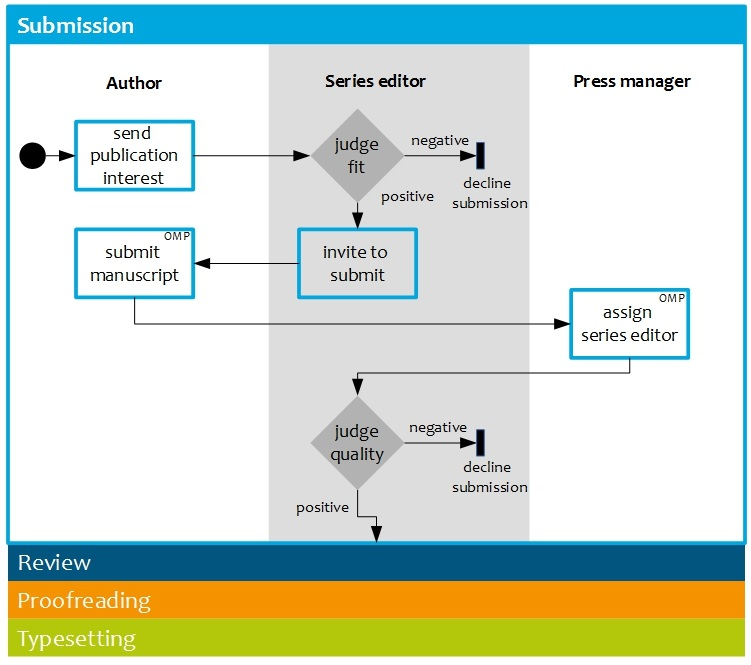
\includegraphics[width=1\textwidth]{./img/workflow_submission.jpg} \caption{Workflow: Submission}
\label{fig:workflowSubmission}
\end{figure}

The workflow (see fig. \ref{fig:workflowSubmission}) starts in general with a publication interest send via mail by the author. Invite the author to submit to your series in OMP, if the topic fits. The author will upload the submission in OMP. The press manager will assign you to the submission and you will be notified. Follow the link in the notification mail or open the submission tab at you dashboard. Under \textit{my assigned submissions} you will find the submission. Click on the title to start. 

\begin{figure}[h] \centering
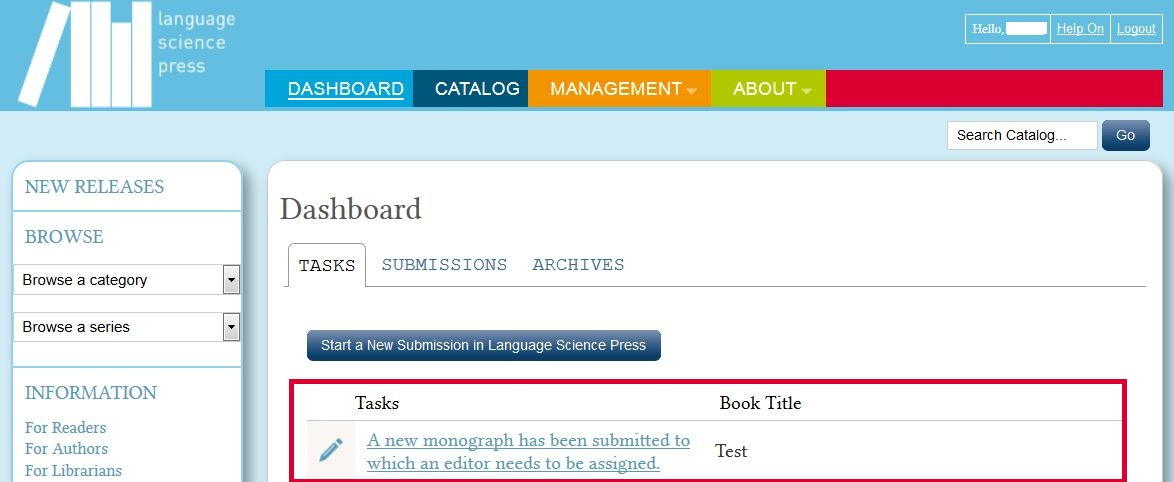
\includegraphics[width=1\textwidth]{./img/editor-1.jpg} \caption{New submission on the dashboard}
\label{fig:editor1}
\end{figure}

% Each workflow stage has access (via the links near the top right corner) to the submission's catalog tool (which will be covered later), to the info tool (to add notes and see the history), and to the participants tool.

% The Info tool allows you to view any notes added to the submission by various participants, notify various participants, and view the overall submission history, including a log of all submission actions and emails.

% The Participants tool allows you to manage all participants associated with the submission: editors, authors, translators, and so on. 

% ++++++++++++++++ instruction for the press manager: how to assing an editor - outsource? +++++++++++++

%\subsection*{Press Manager}

%\begin{figure}[here!] \centering
%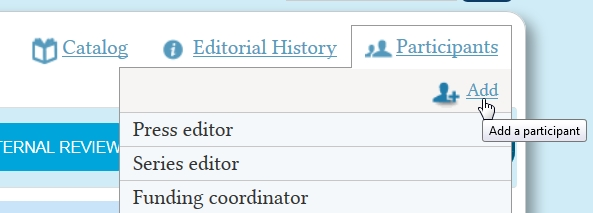
\includegraphics[width=1\textwidth]{./img/addParticipant.jpg} \caption{Add Editor}
%\label{fig:addParticipant}
%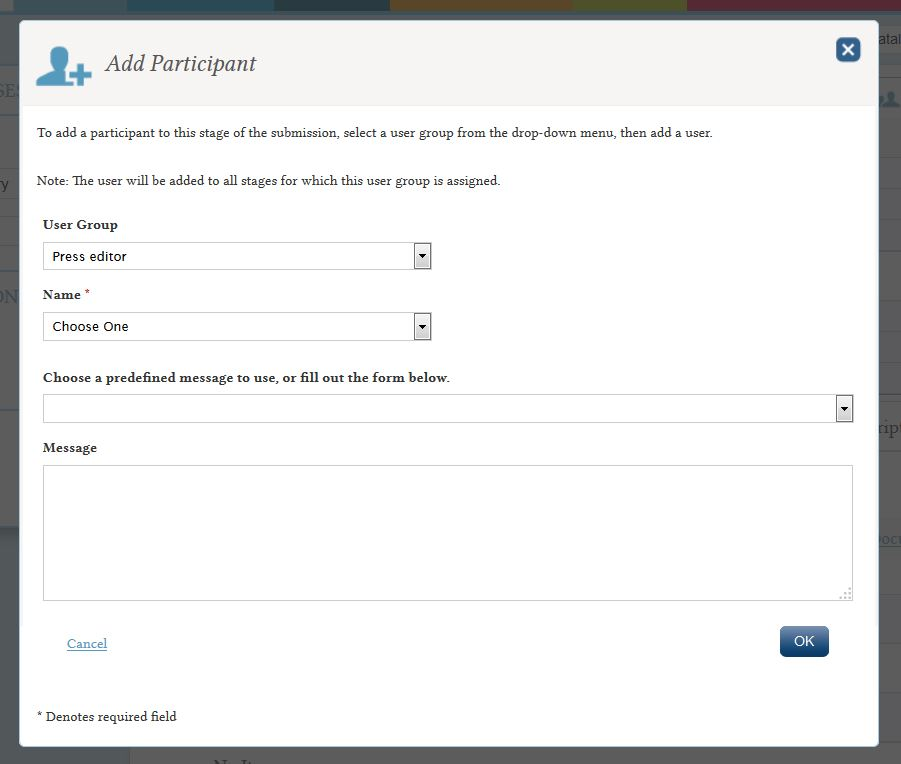
\includegraphics[width=1\textwidth]{./img/addParticipant-1.jpg} 
% \caption{Add Editor}
%\label{fig:addParticipant1}
%\end{figure}

% A press editor and a series editor must be assigned to a submission before the review or editing processes can be initiated. Click the \textit{Participants} link to open the dropdown, click the \textit{Add Participant} link (see fig. \ref{fig:addParticipant}), choose the relevant user group (in this case, either \textit{Series Editor} or \textit{Press Editor}), and choose the user from the list (see fig. \ref{fig:addParticipant1}).

% ++++++++++++++++++++++++++++++++++++++++++++++++

All files provided by the author are available from the first submission workflow page. You can upload additional documents under the \textit{submission documents} section, and these will be available to all users assigned to the submission. When uploading a submission take care to select the type of the document before uploading the file. 

As an editor, you have four options for handling a submission (\figref{fig:options}): 
\begin{enumerate}[noitemsep]
\item send to internal review: editor selects files for review within the press
\item send to external review: editor selects files sent out for review
\item accept submission: editor selects files for editorial stage
\item decline submission: editor archives submission.
\end{enumerate}

\begin{figure}[h] \centering

\includegraphics[width=1\textwidth]{./img/options.jpg} \caption{Options}
\label{fig:options}
\end{figure}

To start an internal or an external review click the matching button and select the submission files the author provided for inclusion in the review process, and optionally upload new files or revise existing files. %(see fig. \ref{fig:internalReview1}). 

%\begin{figure}[here] \centering
%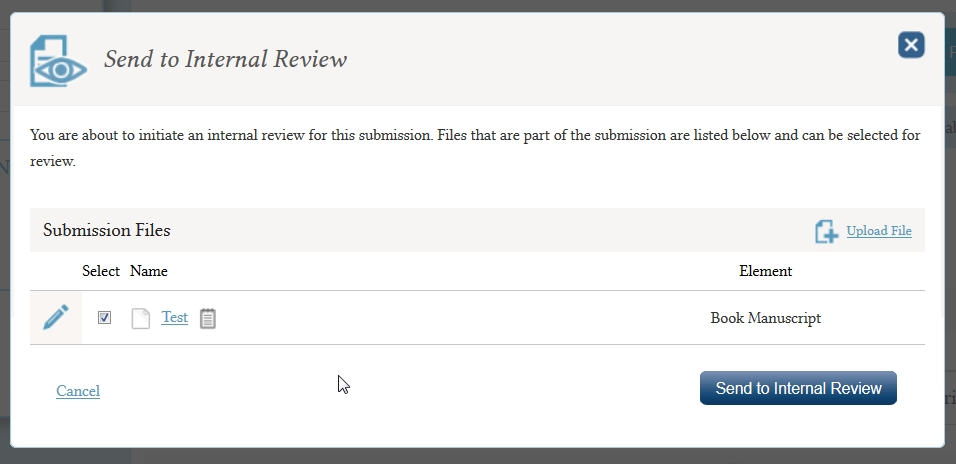
\includegraphics[width=1\textwidth]{./img/internalReview-1.jpg} \caption{Internal Review}
%\label{fig:internalReview1}
%\end{figure}


% *** Review ***

\section{Internal and External Review} 

\begin{figure}[h] \centering
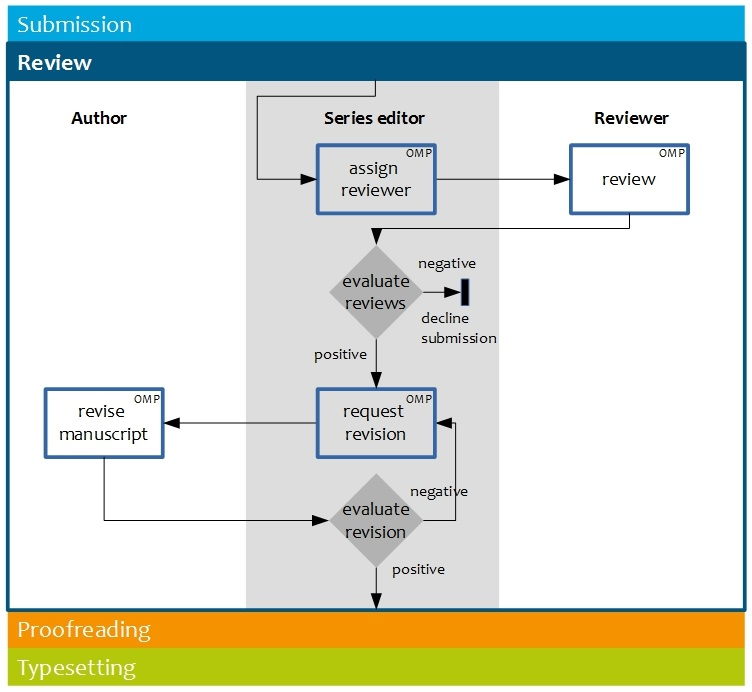
\includegraphics[width=1\textwidth]{./img/workflow_review.jpg} \caption{Workflow:  Review}
\label{fig:review}
\end{figure}

Internal and external Review differ only by target group -- the procedure is the same. The workflow (\figref{fig:review}) applies to both stages. Reviewers associated with the press go over the submission. As editor, you will assign reviewers and, once the reviews are back, assess the reviews and ask the author to revise his manuscript.

\begin{figure}[h] \centering
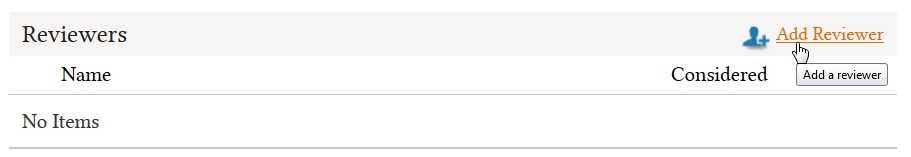
\includegraphics[width=1\textwidth]{./img/addReviewer.jpg} \caption{Internal Review II}
\label{fig:addReviewer}
\end{figure}


Reviewers can be assigned to the submission by clicking \textit{add reviewer} (\figref{fig:addReviewer}). You are able to choose from a pool of already-enrolled reviewers; create a new user as reviewer; enroll new users as reviewers; add a personal message to the review request; set response and review due dates; and choose the review type (blind; double-blind; open). Once reviewers are assigned, you can contact them and revise their due dates by clicking the icon next to their names. %You will be notified of completed reviews, and can access the reviews by clicking on the reviewer's name in the reviewers section.

All author, reviewer and editor revision files are available from the revisions section. Only documents included in this section will be available to be passed on to later workflow stages. Upload the reviewed file to this section (\figref{fig:uploadRevision}).

\begin{figure}[h] \centering
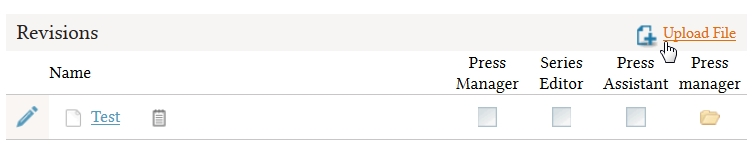
\includegraphics[width=1\textwidth]{./img/uploadRevision.jpg} \caption{Upload Revision}
\label{fig:uploadRevision}
\end{figure}


UP TO HERE

Once all reviews are in, you must make a decision on the submission. You have the following options: 
\begin{figure}[h] \centering

\includegraphics[width=1\textwidth]{./img/internalReview-2.jpg} 
\end{figure}
\begin{itemize}[noitemsep]
\item request revisions: the author will be able to modify their submission information and/or upload revised submission files
% Dies ist immer ein schwieriger Punkt, weil unklar bleiben könnte, ob das Manuskript in jedem Fall nach den Revisions angenommen wird, oder ob es auch noch die Option gibt, dass sie abgelehnt werden, wenn sie die Revisions nicht zufriedenstellend ausführen. Das würde ich hier kurz erläutern. Aus diesem Grund braucht es unbedingt auch Informationen in den Guidelines, die den Review-Prozess für die Autoren-Seite erläutert! - Christina
\item resubmit for review: the submission will enter an entirely new internal review round
\item send to external review: editor selects files to send to the external review process
\item accept for submission: the submission will enter the Editorial stage, bypassing external review
\item decline submission: the submission will be archived and the author notified
\end{itemize}

At the end of the external review or - if you do not need the external review - accept or decline the submission. If you click on \textit{Accpet Submission} you have to select the revised copy to use in the editorial stage, and click \textit{Record Editorial Decision}. You will then be taken to the editorial stage.


%\subsubsection{Undertaking Review}
%\todo[inline, color=green!40]{Do we need "Undertaking Review" or can files be uploaded easier?}
%\todo[inline, color= green!40]{TODO: Rewrite}

% If you have been requested to review a submission, you will find the submission listed in your Dashboard's Tasks page, as well as in your Submissions page (in the My Assigned Submissions queue). To begin the four-step review process, click the submission's title.

% Click through the first two steps and upload the review file at step three.

% Step 1: Request The first step of the review process will provide you with the information you need to accept or decline the review request. You can review various submission details including title and description (and, depending on the review type, author information). Due dates suggested by the editor are also provided. You may click either Decline Review Request or Accept Review.

% Step 2: Guidelines All review guidelines and reference files will be available to you on Step 2 if you have accepted the request. Follow these instructions to complete your review in Step 3. You may return to this page whenever you need to during the review process.

% Step 3: Download + Review The review itself can be completed in Step 3. You can download the submission files for review; submit your review in the provided review form (required); and optionally upload files for the editor and/or author to consult, including revised versions of the original review file(s). Once you have completed your review, click the Submit Review button -- but note that once you have submitted your review you will not be able to modify any aspect of it.

% Step 4: Next Steps The final step is an acknowledgment that the press has received your review. Your review duties are over! 

% *** External Review ***

% At the External Review stage, reviewers external to the press go over the submission. As an editor, you will assign reviewers and give them access to review files and, once the reviews are back, assess the reviews and select the appropriate action: initiate a new review round, request revisions or resubmission, or accept or decline the submission (more details on these actions are below).

% The External Review stage begins with the editor using Upload/Select files to identify the submission files for review.

% Reviewers can be assigned to the submission by clicking the Add Reviewer link. You are able to choose from a pool of already-enrolled reviewers; enroll new users as reviewers; add a personal message to the review request; set response and review due dates; and choose the review type (blind, double-blind, or open). Once reviewers are assigned, you can contact them and revise their due dates by clicking the yellow icon next to their name.

% Once the review has been completed, you will be notified of completed reviews. As editor, you can access the reviews by clicking on the reviewer's name in the Reviewers section.

% All author, reviewer and editor revision files are available from the Revisions section. Only documents included in this section will be available to be moved to later workflow stages.

% Once all reviews are in, you must make a decision on the submission. You may select: 1) Request Revisions, in which case the author will be able to modify their submission information and/or upload revised submission files; 2) Resubmit For Review, in which case the submission will enter an entirely new external review round; 3) Decline Submission, at which point the submission will be archived and the author notified; or 4) Accept Submission, at which point the submission will enter the Editorial stage. These selections are made by clicking on one of the dark blue boxes at the top of the External Review page.

\newpage

% *** Editorial ***

\section{Proofreading} 

\begin{figure}[h] \centering
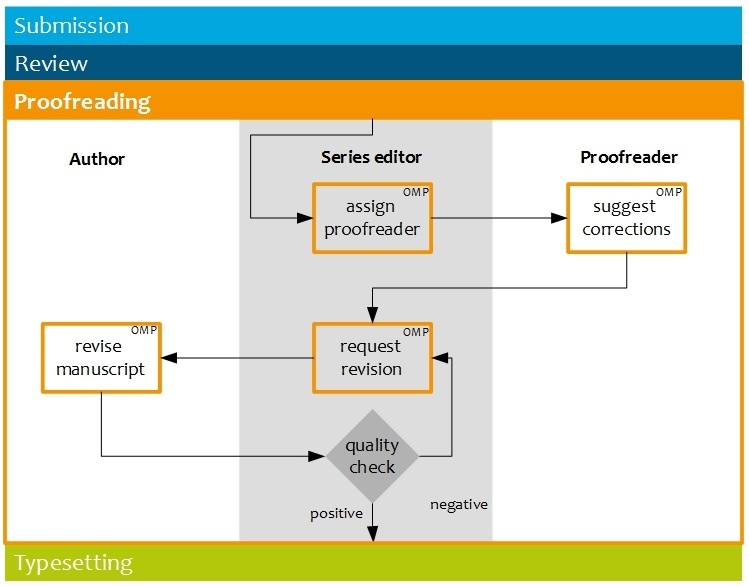
\includegraphics[width=1\textwidth]{./img/workflow_proofreading.jpg} \caption{Workflow: Proofreading}
\label{fig:workflowProofreading}
\end{figure}

The goal of proofreading is to have a fair copy of the manuscript ready to move to production. Series editors, proofreaders and authors are involved in this stage. The series editor manages the process: he assigns the proofreader and returns the corrections to the author for revision (see fig. \ref{fig:workflowProofreading}). Figure \ref{fig:editorial} shows the overview page of the editorial stage. 

\begin{figure}[h] \centering
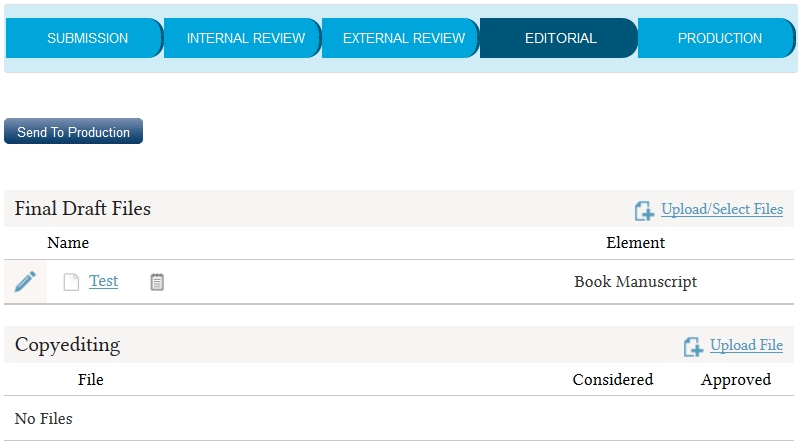
\includegraphics[width=1\textwidth]{./img/editorial.jpg} \caption{Editorial}
\label{fig:editorial}
\end{figure}

\newpage

% \subsubsection*{Editors and the Editorial Process}

Approved submissions are available at \textit{Final Draft Files} and copyedited files may be uploaded to the section \textit{Copyediting} (see fig. \ref{fig:editorial}). Authors and/or editors may be assigned to review the copyedited files and respond to queries. Final copyedited files may then be uploaded, at which point the submission can be sent to the production stage.

To copyedit a file, download the file from the \textit{Final Draft} section and edit it. Then upload it to the \textit{Copyediting} section, and optionally assign one or more users participating in the submission process (for example another editor, or the author) to audit the copyedited file. You may have to assign these users under the \textit{Participants} dropdown before they will be available as auditors.
% Das ist an dieser Stelle eine neue Rolle/Funktion. Was genau ist mit "audit" gemeint? (Im nicht-muttersprachlichen Raum könnte das auch ein schwer zu verstehender Terminus sein). Da der Terminus ja noch weiter verwendet wird, UNBEDINGT ausführlicher erläutern, ggf. schon als Rolle am Anfang vorstellen.


Multiple files may be sent for auditing, and an auditing due date can be set. You will be notified of completed audits, and can access the audits by clicking on the participant's name as it appears under the file. Finally, you will be able to sign off as copyeditor on the audited copyedit file by clicking the checkbox under the Copyeditor column.

After you approved the copyediting files, they can be send to the production stage. Click the \textit{send to production} link (see fig. \ref{fig:editorial}) and select the files you want to send from the list.
% (see fig. \ref{fig:approve})

%\begin{figure}[here] \centering
%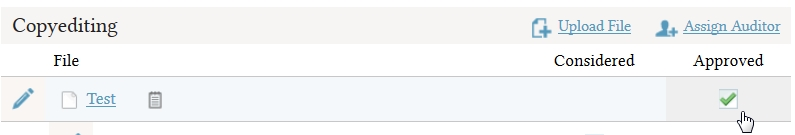
\includegraphics[width=1\textwidth]{./img/approve.jpg} \caption{Approve}
%\label{fig:approve}
%\end{figure}

% +++ outsource? +++++++++++++++++

% \subsubsection*{Auditors and the Editorial Process}

% If you have been asked to audit a file that is being copyedited, you will receive an email indicating this, and the task will also be listed on your Dashboard. To complete the auditing process, go to your Dashboard and click on the audit request. This will bring you to a page where you can download, review and respond to the copyedited file.

% From this page you will be able to download any copyedited files that you have been asked to audit. Download and review the copyedited manuscript, and then click \textit{Upload a Response} to respond to the auditing request and sign off on your audit. You will be able to add any notes you may have regarding the copyedited file, and even upload a revised or annotated copyedited file for the editor to review.

% The assigned editor will receive a notification after you sign off on your auditing duties. 

% ++++++++++++++++++++++++++++++

\newpage

% *** Typesetting ***

\section{Typesetting} 

\begin{figure}[h] \centering
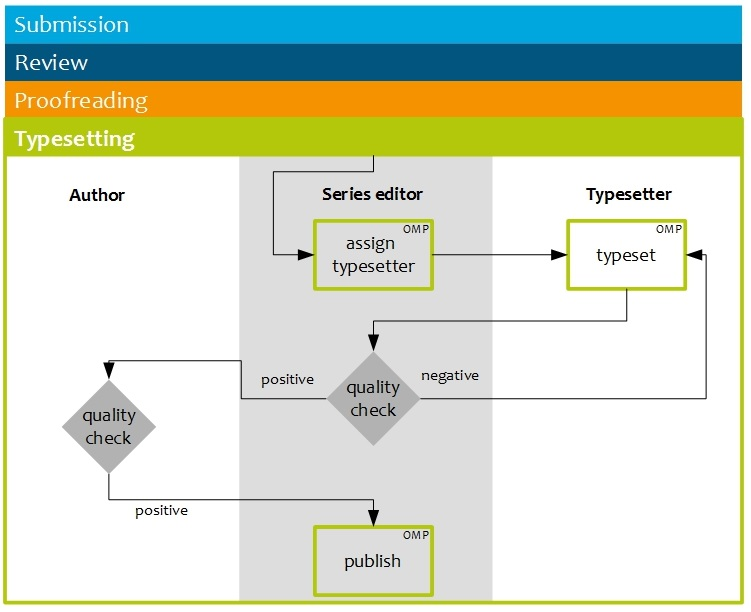
\includegraphics[width=1\textwidth]{./img/workflow_typesetting.jpg} \caption{Typesetting}
\label{fig:workflowTypesetting}
\end{figure}


The submission's production stage with typesetting is generally initiated after the copyediting stage has been completed (in the workflow named as proofreading), although the editor may choose to add information as it becomes available earlier in the workflow process. The production stage is used to create and manage publication formats (e.g. paperback, softcover, PDF, ePub), final publication-ready versions of the submission, and the catalog. 
% This process is normally managed by a production editor, with the input and assistance of designers and proofreaders. Production editors can be assigned using the \textit{Participants} dropdown. 
Figure \ref{fig:production} shows the overwiev page of the production stage.

\begin{figure}[h] \centering
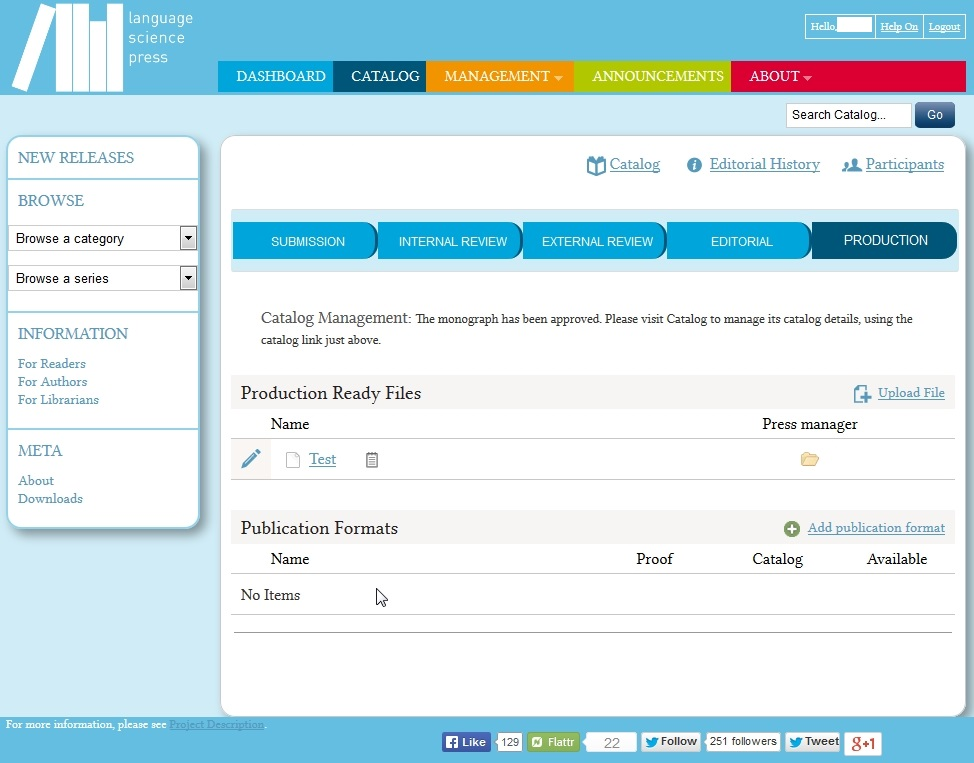
\includegraphics[width=1\textwidth]{./img/production.jpg} \caption{Production}
\label{fig:production}
\end{figure}

%\subsection*{Production editors and the production process}

All approved and copyedited submission files from the editorial stage are available in the \textit{production ready files} section, and additional files can be added if need be (see link \textit{Upload File} in fig. \ref{fig:production}).

The entirety of the submission's information -- including submission placement, metadata, contributors, chapters, and so on -- can be reviewed and edited at the \textit{Catalog} menu (see chapter \ref{sec:catalog}).

Different publication formats (audio, digital, hardback, paperback/softback) can be configured for the submission in the \textit{publication formats} section. Once you have added a format, a new section for that format will be made available to you, and you will be able to upload files there (see fig. \ref{fig:publicationFormats}). After uploading a file you can add an auditor.

\begin{figure}[h] \centering
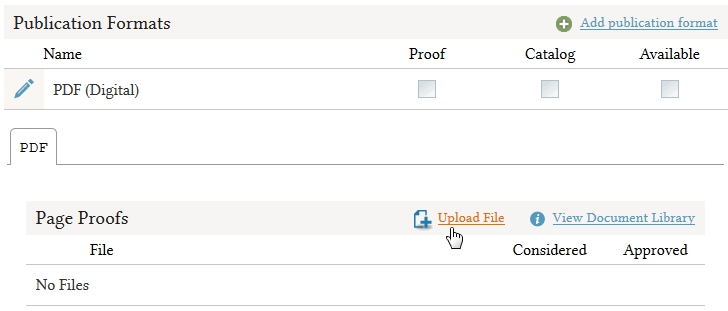
\includegraphics[width=1\textwidth]{./img/publicationFormats.jpg} \caption{publication Formats}
\label{fig:publicationFormats}
\end{figure}

%\subsection*{Auditors and the production process}

%If you have been asked to audit a publication-ready file, you will receive an email indicating this, and the task will also be listed on your Dashboard. To complete the auditing process, go to your Dashboard and click on the audit request. This will bring you to the submission's production page.

%From this page you will be able to download any final publication files that you have been asked to audit. Download and review the manuscript, and then click the checkbox under the Auditor column to sign off on your audit. You will be able to add any notes you may have regarding the file, and even upload a revised or annotated file for the editors to review. The assigned production editor will receive a notification after you sign off on your auditing duties. 

\newpage

% *** Catalog ***

\section{Publication and catalog} \label{sec:catalog}

The public catalog -- the grouping of books available at the press home page -- can be managed in a number of ways. OMP includes an overall catalog management interface which you can find at the navigation bar: management -> catalog. You will also find a Catalog Entry tool available to you for each individual submission, on all of the submission's pages (see fig. \ref{fig:catalog}).

\begin{figure}[h] \centering

\includegraphics[width=1\textwidth]{./img/catalog.jpg} \caption{Open the Catalog Entry of a submission}
\label{fig:catalog}
\end{figure}

Books can be sorted by category and series, both in the catalog management interface, and also on the main home page once published. Authors may assign their original submissions to various categories and series, and editors can change these assignments at any time. 

\subsection*{Managing individual catalog entries}

\begin{figure}[h] \centering
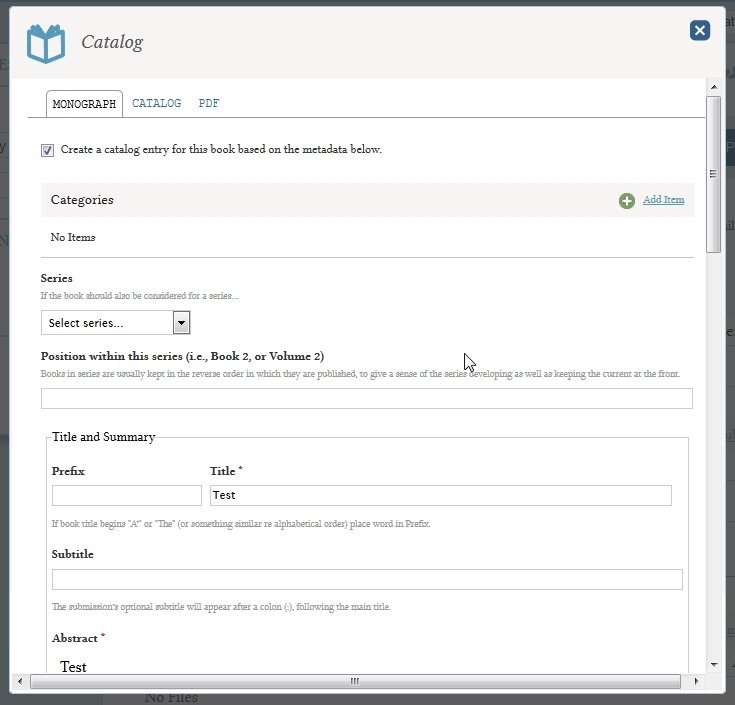
\includegraphics[width=1\textwidth]{./img/metadata.jpg} \caption{The catalog entry management tool}
\label{fig:metadata}
\end{figure}

The catalog entry management tool (see fig. \ref{fig:metadata}) consists of \textit{Monograph} and \textit{Catalog} tabs, as well as additional tabs for each of the publication formats (for e.g., trade paperback, epub, pdf, etc.). The additional tabs will appear once you have added a publication format in the \textit{publication formats} step of the production stage. 

Use the \textit{monograph} tab to modify the book's metadata. This includes title, summary, contributors, coverage, and additional refinements like language, keywords, and supporting agencies. Here you will also be able to specify/modify the submission type (the submission type is usually one of 'image', 'text', or other multimedia types including 'software' and'interactive').

Use the \textit{catalog} tab to modify the book's catalog information. This includes a book cover image, audience information, information on representatives (such as any agents or suppliers) who are not direct members of the press, and publication formats. 

The individual publication format tabs can be used to configure the format itself and make it available on the public catalog. Much of this information can also be disseminated through ONIX extracts.

\subsection*{Publication essentials}

For a manuscript to appear in the public catalog, you must approve the submission's metadata for public display. You can do this from the catalog entry tool's Submissions tab (see fig. \ref{fig:metadata}). Here you will find all of the submission's placement, indexing and authorial information. There is also a checkbox to create a catalog entry (see fig. \ref{fig:metadata} at the top). Checking off this box and saving the form will publish the publication in the public catalog.

For a book's publication formats (e.g. audio, digital, hardback, softback/paperback) to appear in the public catalog listing, you must approve the format's information for public display. You can do this from the catalog entry tool's publication format tabs. Simply open the catalog entry tool; click on the relevant tab (e.g. "Digital"); review the information listed on the resulting page; and check off the checkbox that says "This publication format is ready to be included in the public catalog" and click save.

In order for a digital edition of a book to be available for download, you must:
\begin{itemize}[noitemsep]
\item create a digital format (e.g. ebook) under the production workflow stage;
\item upload files to the format's proof reading step in the production workflow stage;
\item audit and approve all proofs;
\item ensure that the submission and the format type are both marked as available in the catalog.
\end{itemize}
% if charging a fee for the digital edition, ensure that you have a payment method selected under Management -> Distribution Process (either paypal or manual payment); finally, ensure that you configure the Direct Sales Availability + Pricing section for that particular format in the Catalog Entry, where you can either set a particular format as Open Access, or optionally set a fee for purchase.


Figure \ref{fig:publication} shows an example of the catalog page of a published book in OMP.

\begin{figure}[h] \centering
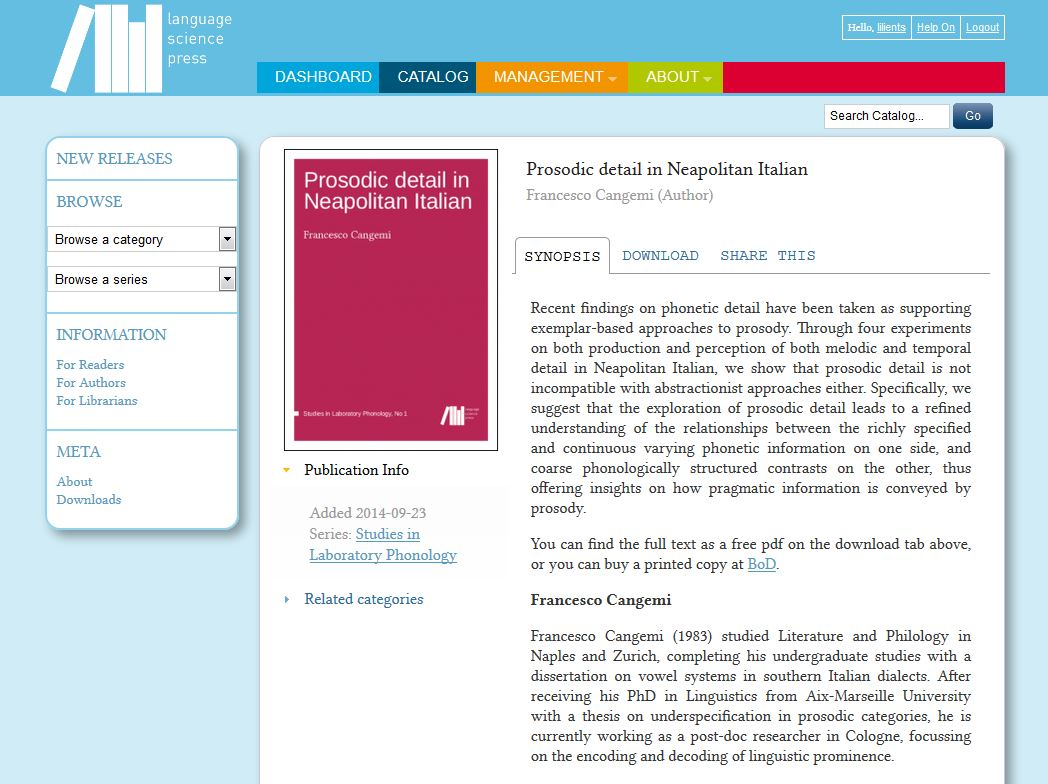
\includegraphics[width=1\textwidth]{./img/publication.jpg} \caption{Publication Example}
\label{fig:publication}
\end{figure}

\newpage
\section{Fast Lane}
As press manager you can publish a document directly after the submission and skip the review and editorial process completely. Hand in the submission as described in chapter \ref{sec:submission}. To publish the submitted document, select \textit{Expedite this submission} at the last step of the submission process (see fig. \ref{fig:fastLane}).

\begin{figure}[h] \centering
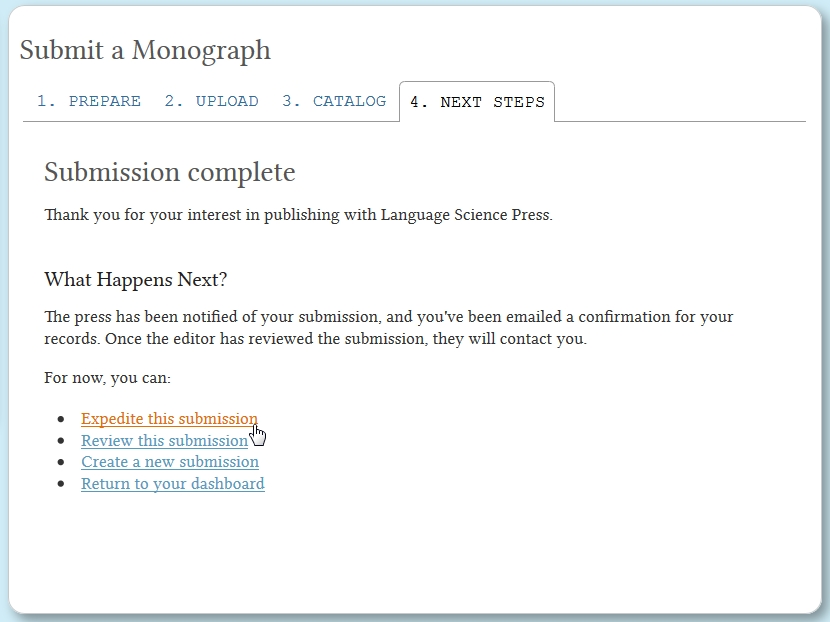
\includegraphics[width=1\textwidth]{./img/fastLane.jpg}
%\caption{Fast Lane}
\label{fig:fastLane}
%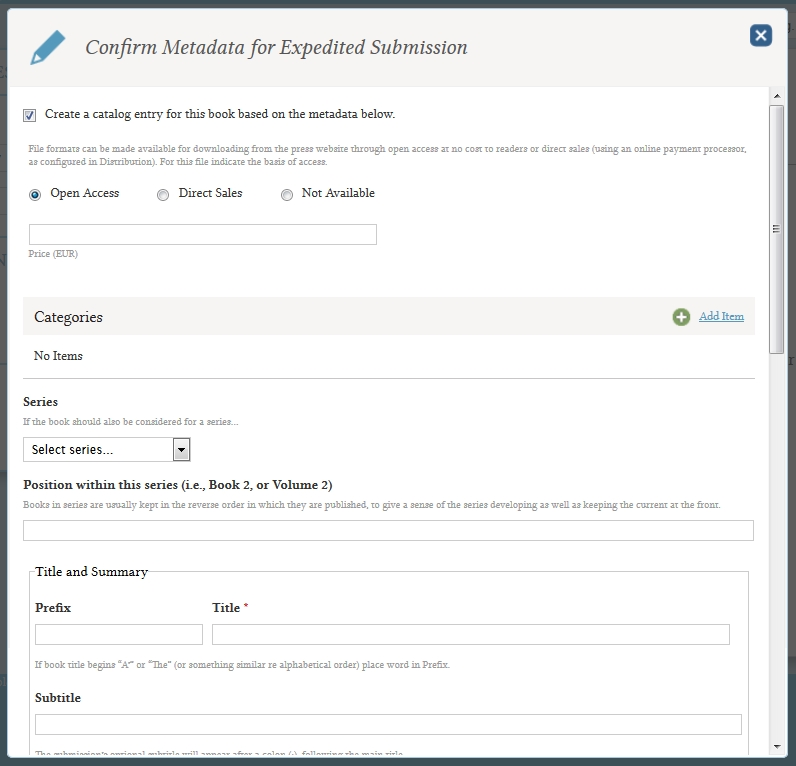
\includegraphics[width=0.8\textwidth]{./img/fastLane-1.jpg} \caption{Fast Lane}
%\label{fig:fastLane1}
\end{figure}

